\documentclass[a4paper,11pt]{article}
\usepackage{amsmath,amsthm,amsfonts,amssymb,amscd,amstext,vmargin,graphics,graphicx,tabularx,multicol} 
\usepackage[francais]{babel}
\usepackage[utf8]{inputenc}  
\usepackage[T1]{fontenc} 
\usepackage{pstricks-add,tikz,tkz-tab,variations}
\usepackage[autolanguage,np]{numprint} 

\setmarginsrb{1.5cm}{0.5cm}{1cm}{0.5cm}{0cm}{0cm}{0cm}{0cm} %Gauche, haut, droite, haut
\newcounter{numexo}
\newcommand{\exo}[1]{\stepcounter{numexo}\noindent{\bf Exercice~\thenumexo} : \marginpar{\hfill /#1}}
\reversemarginpar


\newcounter{enumtabi}
\newcounter{enumtaba}
\newcommand{\q}{\stepcounter{enumtabi} \theenumtabi.  }
\newcommand{\qa}{\stepcounter{enumtaba} (\alph{enumtaba}) }
\newcommand{\initq}{\setcounter{enumtabi}{0}}
\newcommand{\initqa}{\setcounter{enumtaba}{0}}

\newcommand{\be}{\begin{enumerate}}
\newcommand{\ee}{\end{enumerate}}
\newcommand{\bi}{\begin{itemize}}
\newcommand{\ei}{\end{itemize}}
\newcommand{\bp}{\begin{pspicture*}}
\newcommand{\ep}{\end{pspicture*}}
\newcommand{\bt}{\begin{tabular}}
\newcommand{\et}{\end{tabular}}
\renewcommand{\tabularxcolumn}[1]{>{\centering}m{#1}} %(colonne m{} centrée, au lieu de p par défault) 
\newcommand{\tnl}{\tabularnewline}

\newcommand{\bmul}[1]{\begin{multicols}{#1}}
\newcommand{\emul}{\end{multicols}}

\newcommand{\trait}{\noindent \rule{\linewidth}{0.2mm}}
\newcommand{\hs}[1]{\hspace{#1}}
\newcommand{\vs}[1]{\vspace{#1}}

\newcommand{\N}{\mathbb{N}}
\newcommand{\Z}{\mathbb{Z}}
\newcommand{\R}{\mathbb{R}}
\newcommand{\C}{\mathbb{C}}
\newcommand{\Dcal}{\mathcal{D}}
\newcommand{\Ccal}{\mathcal{C}}
\newcommand{\mc}{\mathcal}

\newcommand{\vect}[1]{\overrightarrow{#1}}
\newcommand{\ds}{\displaystyle}
\newcommand{\eq}{\quad \Leftrightarrow \quad}
\newcommand{\vecti}{\vec{\imath}}
\newcommand{\vectj}{\vec{\jmath}}
\newcommand{\Oij}{(O;\vec{\imath}, \vec{\jmath})}
\newcommand{\OIJ}{(O;I,J)}


\newcommand{\reponse}[1][1]{%
\multido{}{#1}{\makebox[\linewidth]{\rule[0pt]{0pt}{20pt}\dotfill}
}}

\newcommand{\titre}[5] 
% #1: titre #2: haut gauche #3: bas gauche #4: haut droite #5: bas droite
{
\noindent #2 \hfill #4 \\
#3 \hfill #5

\vspace{-1.6cm}

\begin{center}\rule{6cm}{0.5mm}\end{center}
\vspace{0.2cm}
\begin{center}{\large{\textbf{#1}}}\end{center}
\begin{center}\rule{6cm}{0.5mm}\end{center}
}



\begin{document}
\pagestyle{empty}
\titre{Interrogation: Fractions }{Nom :}{Prénom :}{Classe}{Date}



\exo{2,5}\\

\q Écrire chaque fraction en toutes lettres :\\

\qa $\dfrac{103}{1000}$ : . . . . . . . . . . . . . . . . . . . . . . . . . . . . . . . . . . . . . . . . . . . .\\

\qa $ \dfrac{18}{3}$ : . . . . . . . . . . . . . . . . . . . . . . . . . . . . . . . . . . . . . . . . . . . .\\

\q Écrire sous forme de fractions :

\bmul{2}

\initqa \qa quatre-vingts neuvièmes : . . . . . . . . .\\


\qa huit quarts : . . . . . . . . .\\

\columnbreak

\qa quatre vingt-neuvièmes : . . . . . . . . .\\

\qa trois demis : . . . . . . . . .\\

\emul

\q Mon numérateur est le double de celui de $ \dfrac{5}{7}$ mon dénominateur est le tiers de celui de $\dfrac{6}{9}$.\\
Je suis . . . . . . . . . . . . . . . . . . . . . . . . .\\


\exo{3} Fractions et partage\\

\initq \q Pour chaque figure, indiquer la fraction de la
surface totale qui est colorée.\\

\begin{center}
\includegraphics[scale=0.75]{fractions1.eps} \\
\end{center}

\begin{center}
\includegraphics[scale=0.6]{fractions3.eps} \includegraphics[scale=0.65]{fractions2.eps} 
\end{center}

\q Hachure une surface représentant :

\bmul{2}

\initqa \qa les $\dfrac{6}{8} $ de l'aire du rectangle :\\


\includegraphics[scale=1]{fractions4.eps} 

\columnbreak

\qa  les $\dfrac{7}{4} $ de l'aire du rectangle :\\


\includegraphics[scale=1]{fractions4.eps} 

\emul

\newpage

\exo{2} Fractions et demi-droite graduée \\

\initq \q Donner les abscisses des points A, B, C et D sous forme de fractions.\\

\includegraphics[scale=0.5]{fractions6.eps} 


\q Sur la demi-droite graduée ci-dessous, placer les fractions suivantes : \hspace*{0.3cm} $\dfrac{2}{6}$\hspace*{0.1cm},\hspace*{0.1cm} $\dfrac{5}{3}$\hspace*{0.1cm},\hspace*{0.1cm} $\dfrac{7}{6}$\hspace*{0.1cm},\hspace*{0.1cm} $\dfrac{3}{2}$\\

\includegraphics[scale=0.45]{fractions5.eps} \\


\exo{2.5}\\

\initq \q Donner le résultat sous forme de fractions :\\

\initqa \qa Les quatre sixièmes de 11 : . . . . . . . . . . . . . . . . . . . . . . . . . . . . . . . . . .\\

\qa Les cinq quarts de 1 000 : . . . . . . . . . . . . . . . . . . . . . . . . . . . . . . . . . . . .\\


\q Claire a dépensé les deux cinquièmes des 55 euros se trouvant dans sa tirelire. Quelle somme a-t-elle dépensée ? \\

\noindent \reponse[2]\\


\q Delphine a bu les trois quarts des 2 litres de lait. Quel volume cela représente-t-il ?\\

\noindent \reponse[2]\\


\q Isabelle a parcouru les trois septièmes des 7,7 km de son parcours quotidien. Quelle distance lui reste-t-il à parcourir ?\\

\noindent \reponse[2]\\



\end{document}
